\section{Conclusões}

A prática permitiu compreender melhor os filtros ativos, em especial uma categoria de filtros ativos chamados de Butterworth, que usa o amplificador operacional na saída, como Buffer. Dessa forma, vimos a aplicação para filtros de primeira e segunda ordem seus efeitos aplicando uma tensão senoidal na entrada. Utilizando para construção da curva de transferência destes dois tipos de filtros.

Apesar das dificuldades teóricas oriundas da complexidade teórica do circuito, a prática foi executada sem mais problemas, permitindo comprovar a teoria a partir dos resultados práticos.

A importância desse tipo deste circuito se reflete por toda a engenharia elétrica, sondando diversas aplicações, que vão desde a modulação na engenharia de telecomunicações até a utilização em um circuito complexo em eletrônica.

\newpage

\section{Anexos}

\vspace{60pt}
\begin{figure}[htbp!]
    \centering
    \vspace{16cm}
		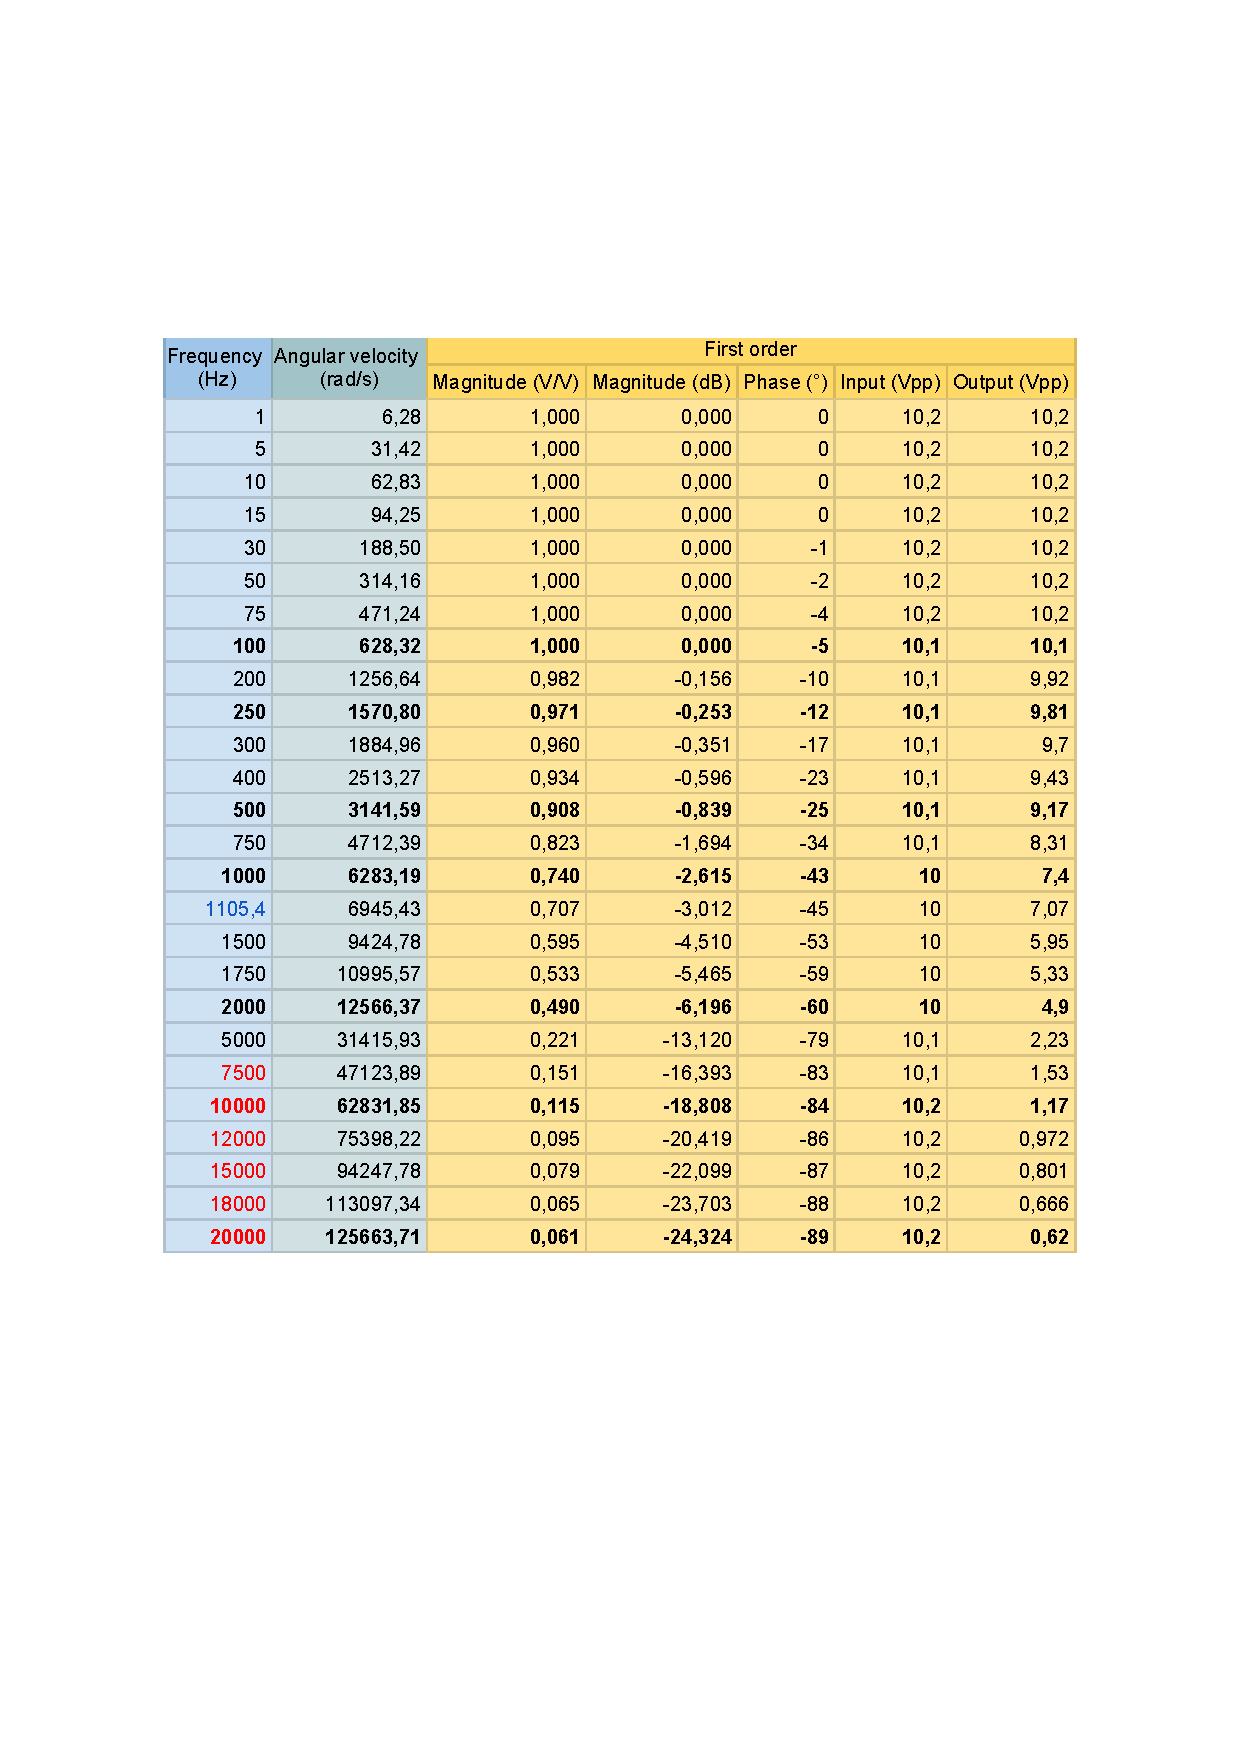
\includepdf[page={1}]{first_order.pdf}  
	\caption{Tabela contendo os valores medidos na prática para o filtro passa-baixa de 1ª ordem.}
	\label{table:1}
\end{figure}

\newpage

\begin{figure}[htbp!]
	\centering
	\vspace{19cm}
	    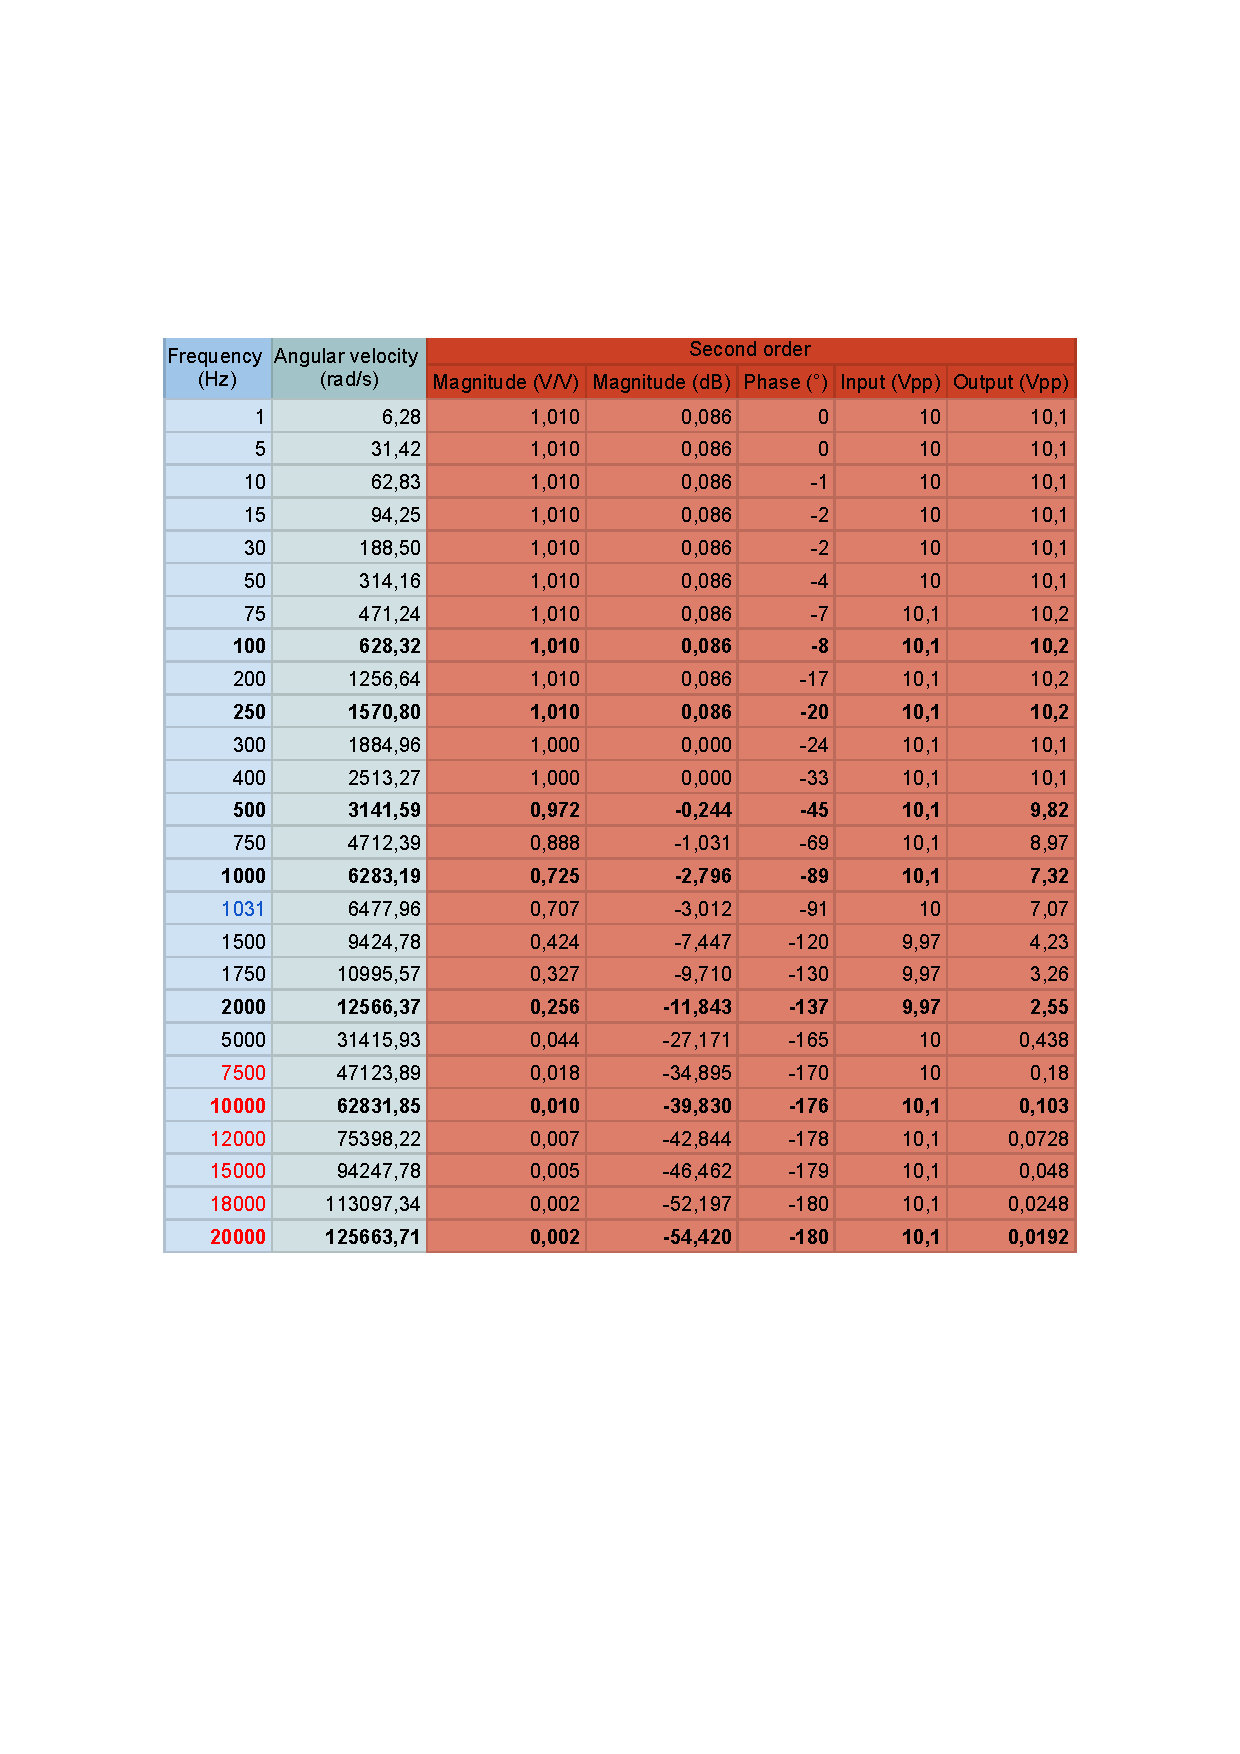
\includepdf[page={1}]{second_order.pdf} 
	\caption{Tabela contendo os valores medidos na prática para o filtro passa-baixa de 2ª ordem.}
	\label{table:2}
\end{figure}
